\documentclass[a4paper, 11pt]{article}
\usepackage{lmodern}
\usepackage[top=30mm, bottom=35mm, left=25mm, right=25mm]{geometry}
\usepackage{fancyhdr, graphicx}
\usepackage{amsmath}
\usepackage{amsthm}
\usepackage{fancyvrb}
\usepackage[pagebackref=false,colorlinks,linkcolor=blue,citecolor=blue]{hyperref}
\usepackage{longtable}
\usepackage{enumitem}
\linespread{1.6}
\usepackage{comment}
\usepackage{titling}
\pagestyle{fancy}
\fancyhead[L]{}
\fancyhead[R]{\it{\thetitle}}
\setlength{\headheight}{27pt}

\title{Simulink Network Emulator \\ {Manual \& Documentation}}
\author{M. Farzan}
\date{\today}
\begin{document}
\maketitle
\section*{Change-log}
\شروع{لوح}[h]
\تنظیم‌ازوسط
\شروع{جدول}%
{p{2cm}p{2cm}p{2.5cm}p{7cm}}
نسخهٔ سند & نسخهٔ کد & تاریخ نگارش & تغییرات \\
\hline
۱ & \ورب{1.0} & ۹۹/۱۲/۲۱ & [اولین نسخه]
\پایان{جدول}
\پایان{لوح}

\tableofcontents
\newpage
\section{Introduction}
Simulink network emulator block simulates network effects. The current features include:
\begin{itemize}
\item Sampling continuous input with configurable rate
\item Simulating latency with constant value or Gaussian distribution
\item Simulating packet reordering due to jitter
\item Simulating packet loss with two models that include (a) independent random and (b) 4-state Markov chain
\end{itemize}

\section{Definitions}
The following definitions are used throughout this document:
\begin{itemize}
\item[] \textbf{Latency}: The time difference from sending the first bit of a packet from source system to receiving the last bit of that packet in destination system. In case that the packet is not received at destination, the value is undefined. \cite{rfc7679}
\item[] \textbf{Packet loss}: A value of either 0 or 1. The value of 0 denotes a packet that is received and a value of 1 denotes a packet that is not received. \cite{rfc7680}
\item[] \textbf{Latency variation}: The difference of two latencies. \cite{rfc3393}
\item[] \textbf{Packet reordering}: Packet reordering assigned to a packet with sequence number of $s$ is TRUE if and only if when the packet is received at destination, it holds that $s<\textrm{NextExp}$ where NextExp equals the expected sequence number. \cite{rfc4737}
\end{itemize}

\section{Installation Guide}
\begin{enumerate}
\item Download the last version of the package from \href{https://github.com/m2-farzan/simulink-network-emulator/releases/latest/download/IDAS-Network-Emulator.mltbx}{this link}.
\item Open MATLAB and from the file browser panel, open the download folder.
\item In the file browser panel, double-click on \Verb~IDAS-Network-Emulator.mltbx~.
\item In the window that shows up, click on ``Install''.
\item Now the library should be installed. To verify, open Simulink Library Browser. If it is already open, press F5 button.
\item In case of a successful installation, there should be a new item in the toolbox list named ``IDAS Network Emulator'' (fig. \ref{good-install})
\begin{figure}[h]
\centering
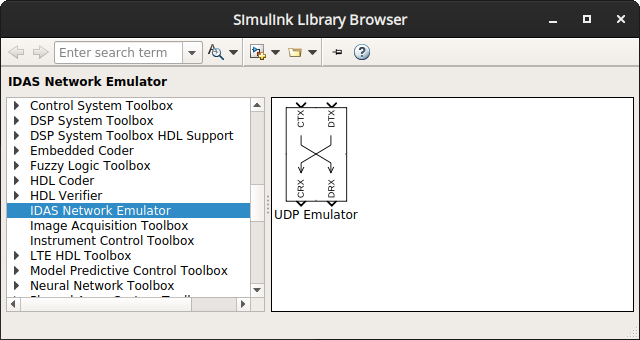
\includegraphics[width=12cm]{img/good-install}
\caption{Successful installation}
\label{good-install}
\end{figure}
\end{enumerate}

\section{Usage Guide}
Before using the block, make sure that the model solver is configured to use variable steps. This holds in the default settings, so you should be okay if you have not changed it.
\begin{enumerate}
\item Drag ``UDP Emulator'' block into your model.
\item Establish the required connections. The block has two channels, one for sending data from cloud (C) to device (D) and the other one for returning data from device (D) to cloud (C). The block ports are labeled as follows:
\begin{itemize}
\item[] \textbf{CTX}: Data that cloud sends to internet.
\item[] \textbf{DRX}: Data that device receives from internet.
\item[] \textbf{DTX}: Data that device sends to internet.
\item[] \textbf{CRX}: Data that cloud receives from internet.
\end{itemize}
After setting connections, the model should look life fig. \ref{model}. Note that it is not required for both channels to be connected---communication can be one directional. Also, note that in the cases where multiple signals are needed to go through network, it is required to convert them into one vector signal (using ``Vector Concatenate'' block) before feeding the result to network block. The signal that comes out can be de-concatenated using ``Submatrix'' block. An example of this is located at examples/VectorMode.
\begin{figure}[h]
\centering
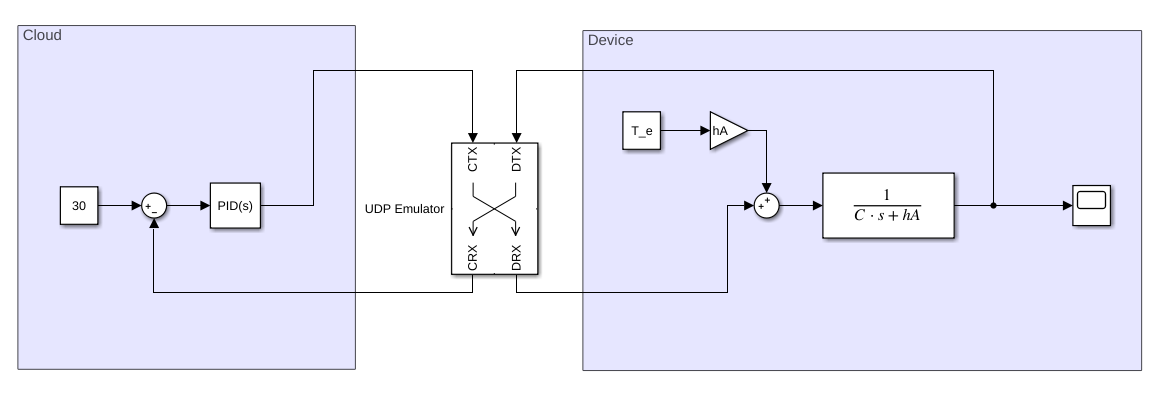
\includegraphics[width=16cm]{img/model.png}
\caption{Correct connection of blocks to the network (This file is available at examples/RemotePidController).}
\label{model}
\end{figure}
\item Double-click on the block to open parameters dialog (fig. \ref{dialog}). Set the parameters with regard to the following table:
\begin{longtable}{l|p{12cm}}
\multicolumn{1}{c|}{Parameter} & \multicolumn{1}{c}{Description} \\
\hline
Cloud sampling interval & This field sets the time interval of sampling the cloud to device signal. In the future, an event-driven mode will be added to support sending discrete commands immediately as a change is detected. \\ \hline
Device sampling interval & Same as above, for device to cloud signal. \\ \hline
Mean Delay & Average packet delay \\ \hline
Delay standard variation & If set to a positive value, packets delays will become random with Gaussian distribution where standard variation of probability function will be equal to the value of this parameter. \\ \hline 
Loss Model & Selects packet loss model which has two options:
\begin{itemize}
\item Independent Random: In this mode, the probability of packet loss for each packet is independent of the others. The parameter of this mode is as follows:
\begin{itemize}
\item Loss probability: The probability of losing each packet
\end{itemize}
\item 4-State Markov Chain: In this mode, a more realistic model is used which is stateful, and can simulate loss ``burst''s. The parameters of this model include:
\begin{itemize}
\item Loss probability ($P_\textrm{loss}$)
\item Mean burst length ($E(B)$)
\item Loss density within the burst ($\rho$)
\item Isolated loss probability ($P_\textrm{isol}$)
\item Mean good burst length ($E(GB)$)
\end{itemize}
Note that the parameters should satisfy the following conditions, otherwise parameters dialog will show an error.
\begin{itemize}
\item $E(B) \ge 1/\rho$
\item $P_\textrm{isol} \le P_\textrm{loss} < \rho$
\item $P_\textrm{loss} - P_\textrm{isol} \le E(B) (1-P_\textrm{isol})(\rho - P_\textrm{loss})$
\item $E(GB) \ge 1$
\item $E(GB) \ge (1-\rho)/\rho$
\item $P_\textrm{isol} \le 1/2$
\end{itemize}
\end{itemize}
\end{longtable}
\begin{figure}
\centering
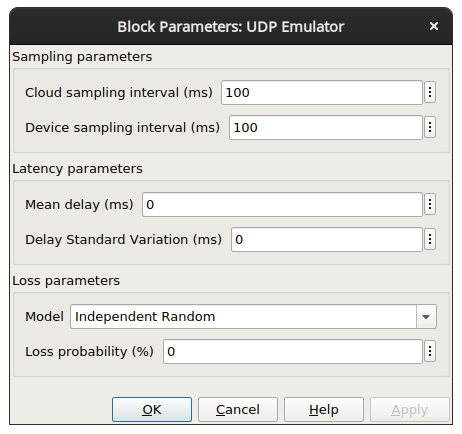
\includegraphics[width=8cm]{img/params-dialog.png}
\caption{Parameters dialog}
\label{dialog}
\end{figure}
\end{enumerate}

\section{Implementation Report}
\subsection{Selected Models}
Packet delays are modeled as a Poisson process, i.e. each packet delay is independent of other packet delays. This assumption is an over-simplification in some use cases, however it has also proven good enough in some studies \cite{Dahmouni2012}. Packet delays are generated randomly with a normal distribution, with the mean value and standard deviation defined as block parameters.

To simulate packet loss, two models are implemented. In the ``Independent Random'' model, packet loss is modeled as a Poisson process. This model is also known as ``Bernoulli model''. This model has only one parameter that defines packet loss probability. The model is simple but in real life, packet loss often has more complex patterns.

In the ``4-State Markov Chain'' packet loss model, network is modeled as a system with 4 possible states. The probability of transition from one state to the other is a defined parameter. This model can simulate loss ``bursts'', and is a generalization of some well-known models including Bernoulli, Simple Gilbert, Gilbert and Gilbert-Elliot \cite{Ludovici2012}. This model is also implemented in ``tc-netem'' tool, which is part of the Linux kernel.

The parameters of 4-State Markov Chain model is its most basic form, are the probabilities of transition between each two states. However, since these parameters are not very intuitive, the network emulator block uses the ``General Intuitive'' parameters suggested in \cite{Ludovici2012}. These parameters translate to vanilla 4-State Markov Chain parameters using the equations that can be found in the mentioned reference.

\subsection{Patterns}
Network emulator block is based on ``Level-2 S-Function'' blocks, with the code being written in MATLAB language. The block reads input ports at sampling ticks. Then, it applies the Markov chain rules to determine if the packet will be lost or not. If the packet is determined not to be lost, the delay value is generated. Then, the packet contents and its delivery time is stored in an array, and the block enters sleep until the next sampling tick, or the next packet delivery time (depending on which one is closer).

\bibliographystyle{vancouver}
\bibliography{ref}
\end{document}
